% !TeX spellcheck = en_GB
\section{Challenges}\label{Challenges}
While building the generic version of Hibernate Search, we will encounter some challenges. We will now discuss the biggest ones and introduce a small example project. This project will be used to showcase some problems and usages later on in this thesis as well.

\subsection{The example project}
Consider a software built with JPA (in this case EclipseLink) that is used to manage the inventory of a bookstore. It stores information about the available books and the corresponding authors. Each author can be related to zero or more Books and each Book can be written by one or more Authors. The entity relationship model diagram looks like this:
\\
\begin{figure}[ht]
	\centering
	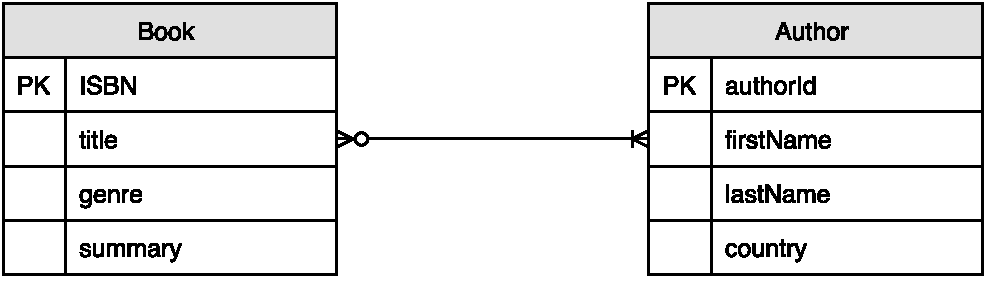
\includegraphics[scale = 0.9]{images/Sample_Project_ER.pdf}
	\caption{the bookstore entity relationship model}
	\label{fig3}
\end{figure}
\\
Using a mapping table for the M:N relationship of Author and Book, the database contains three tables: Author, Book and Author\_Book. The JPA annotated classes for these entities look like this:

\textcolor{red}{Hier Klassen einfügen, und oben im Text erklären, was getan wurde, column definitions alle in JPA machen}

\subsection{indexing \& searching}
Hibernate Search's engine wasn't designed to be used directly by an application developer. Its main purpose is to serve as an integration point for other APIs that need to leverage its power to index arbitrary object graphs annotated with some additional information and query the index for hits. This is why we have to write our own standalone module based on the "hibernate-search-engine" to ease its general usage. After that, we will build an integration of this standalone version with JPA to mimic the behaviour of Hibernate Search ORM as good as possible.

\subsection{index rebuilding}
If the way objects are indexed changes, the existing files have to be purged and recreated in the new index format. The naive approach would be purging the index and then indexing all data sequentially as they are retrieved from the database:
\\
\lstset{language=java}
\begin{lstlisting}[frame=htrbl, caption={naive index rebuilding}, label={lst:naiveIndexing}]
EntityManager em = ...;
<Hibernate Search Controller> search = ...;

search.purgeAll(Book.class);

Query query = em.createQuery("SELECT b FROM Book b");
List<Book> booksFromDb = query.getResultList();
for(Book b : booksFromDb) {
	search.index(b);
}
\end{lstlisting}
While this might work for small databases, bigger datasets will cause this algorithm to run out of memory, since we just retrieve all the data at once. This could be fixed by implementing a batching strategy, but it would still be quite slow as it only uses one thread which would mostly be used for I/O from the database.
\\\\
This is not optimal, since a index rebuild should be as fast as possible because the application cannot be properly used while the job is running. Therefore we need to create a parallel indexing mechanism, just like Hibernate Search ORM has one.

\subsection{automatic index updating}
The most important feature to be re-built is the automatic index updating feature. In Hibernate Search ORM, every change in the database is automatically reflected in the index. It is important to have this feature, because otherwise, developers would have to manually make sure the index is always up-to-date. While this could be done by hiding all the database access logic behind a service layer, even such a solution would be hard to keep error-free as for big applications such a layer will probably not have only a single point of access either.
\\\\
The original Hibernate Search ORM is achieving an up-to-date index by listening to specific Hibernate ORM events that cover all of C\_UD (CREATE, UPDATE DELETE). These events also cover entity relationship collections (for example represented by mapping tables like Author\_Book). As our goal is to create a generic Hibernate Search engine that works with only the JPA interfaces, we cannot rely on any vendor specific event system. Thus, a different solution has to be found.
\\\\
\textcolor{red}{Hier evtl. noch die verschiedenen Möglichkeiten vorstellen? Eigentlich gehören die ja doch später in ihr eigenes Kapitel oder nicht?}

\pagebreak